\documentclass[]{article}

\usepackage{amsmath}
\usepackage{graphicx}
\usepackage{esdiff}
\graphicspath{.}

%opening
\title{Double Pendulum: Theory}
\author{Ben Hoberman}

\begin{document}
	
\date{June 17, 2017}
\maketitle

\section{Introduction}
As it turns out, the double pendulum is pretty complex. For now, I am modeling a double pendulum consisting of two identical sticks, one attached to a fixed anchor and the other attached to the other end of the anchored stick. Some research divulged that Lagrangian mechanics would yield an easier way to understand the motion of this system, so after some research and an MIT online lecture, here is my attempt at using Lagrangian mechanics to describe the behavior of this system:

\section{Describing the System}
\begin{figure}[h!]
	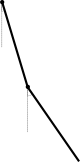
\includegraphics[height=5cm]{situation}
	\caption{A crude image of this double pendulum}
\end{figure}
Each of the sticks of this pendulum has length $\ell$ and mass $m$. $\theta_1$ represents the rotation of the stick attached to the anchor with respect to the vertical, and $\theta_2$ represents the rotation of the other stick, also relative to the vertical. In order to write the Lagrangian for this system, we need to find a way to express its kinetic and potential energies. We will be using $\theta_1$ and $\theta_2$ as the two coordinates that describe this system, so we will work to express everything in terms of $\theta$'s.

The two sticks are the only elements of the system that account for its kinetic energy. Each stick has a component of linear and rotational kinetic energy, $\frac{1}{2}mv^2$ and $\frac{1}{2}I\dot{\theta}^2$. The rotational energy is with respect to the center of mass of each stick.

In order to calculate the speed of the center of mass of each stick, we must do some math. The cartesian coordinates of the centers of mass of the two sticks are as follows:
\begin{gather*}
x_1 = \frac{\ell}{2}\sin(\theta_1) \\
y_1 = -\frac{\ell}{2}\cos(\theta_1) \\
x_2 = \ell \sin(\theta_1) + \frac{\ell}{2} \sin(\theta_2) = \ell (\sin(\theta_1) + \frac{1}{2}\sin(\theta_2)) \\
y_2 = -\ell \cos(\theta_1) - \frac{\ell}{2} \cos(\theta_2) = -\ell (\cos(\theta_1) + \frac{1}{2} \cos(\theta_2))
\end{gather*}
In order to find the linear velocity , we can use the good old Pythagorean theorem to figure out that $v = \sqrt{\dot{x}^2 + \dot{y}^2}$, or, even more conveniently, that $v^2 = \dot{x}^2 + \dot{y}^2$ for each stick. Let's do that:
\begin{gather*}
	v_1^2 = \dot{x_1}^2 + \dot{y_1}^2 = (\dot{\theta_1} \frac{\ell}{2}\cos(\theta_1))^2 + (\dot{\theta_1} \frac{\ell}{2}\sin(\theta_1))^2 = \dot{\theta_1}^2 \frac{\ell^2}{4} \cdot (\cos^2(\theta_1) + \sin^2(\theta_1)) = \dot{\theta_1}^2 \frac{\ell^2}{4} \\
	v_2^2 = \dot{x_2}^2 + \dot{y_2}^2 = \ell^2(\dot{\theta_1}^2 \cos^2(\theta_1) + \frac{\dot{\theta_2}^2}{4}\cos^2(\theta_2) + \dot{\theta_1}\dot{\theta_2}\cos(\theta_1)\cos(\theta_2) \\ + \ell^2(\dot{\theta_1}^2\sin^2(\theta_1) + \frac{\dot{\theta_2}^2}{4}\sin^2(\theta_2) + \dot{\theta_1}\dot{\theta_2}\sin(\theta_1)\sin(\theta_2)) \\
	= \ell^2 (\dot{\theta_1}^2 + \frac{\dot{\theta_2}^2}{4} + \dot{\theta_1}\dot{\theta_2}\cos(\theta_1 - \theta_2)) \\
	v_1^2 + v_2^2 = \ell^2(\frac{5}{4}\dot{\theta_1}^2 + \frac{1}{4}\dot{\theta_2}^2 + \dot{\theta_1}\dot{\theta_2}\cos(\theta_1 - \theta_2)) \\
	K_{linear} = \frac{1}{2}mv_1^2 + \frac{1}{2}mv_2^2 = \frac{1}{2}m(v_1^2 + v_2^2) = \frac{1}{2}m\ell^2(\frac{5}{4}\dot{\theta_1}^2 + \frac{1}{4}\dot{\theta_2}^2 + \dot{\theta_1}\dot{\theta_2}\cos(\theta_1 - \theta_2)) \\ = \frac{1}{8}m\ell^2(5\dot{\theta_1}^2 + \dot{\theta_2}^2 + 4\dot{\theta_1}\dot{\theta_2}\cos(\theta_1 - \theta_2))
\end{gather*}
Because out selected independent coordinates describing the system are $\theta_1$ and $\theta_2$, describing the rotational kinetic energy of the system is much more simple. For each stick, $K_{rot} = \frac12 I \dot{\theta}^2 = \frac12 I (\dot{\theta_1}^2 + \dot{\theta_2}^2)$. Each stick's moment of inertia about its center of mass is $\frac{1}{12} m \ell^2$, so $K_{rot} = \frac{1}{24}m\ell^2(\dot{\theta_1}^2 + \dot{\theta_2}^2)$.

We can now find the total kinetic energy of the system:
\begin{gather*}
	K = K_{linear} + K_{rot} = \frac{1}{8}m\ell^2(5\dot{\theta_1}^2 + \dot{\theta_2}^2 + 4\dot{\theta_1}\dot{\theta_2}\cos(\theta_1 - \theta_2)) + \frac{1}{24}m\ell^2(\dot{\theta_1}^2 + \dot{\theta_2}^2) \\
	= \frac{1}{24}m\ell^2(15\dot{\theta_1}^2 + 3\dot{\theta_2}^2 + 12\dot{\theta_1}\dot{\theta_2}\cos(\theta_1 - \theta_2) + \dot{\theta_1}^2 + \dot{\theta_2}^2) \\
	= \frac{1}{24}m\ell^2(16\dot{\theta_1}^2 + 4\dot{\theta_2}^2 + 12\dot{\theta_1}\dot{\theta_2}\cos(\theta_1 - \theta_2) ) \\
	= \frac16m\ell^2(4\dot{\theta_1}^2 + \dot{\theta_2}^2 + 3\dot{\theta_1}\dot{\theta_2}\cos(\theta_1 - \theta_2))
\end{gather*}

\end{document}
